\documentclass[10pt,a4paper]{article}
\usepackage[utf8]{inputenc}
\usepackage{amsmath}
\usepackage{amsfonts}
\usepackage{amssymb}
\usepackage{graphicx}
\usepackage{epstopdf}
\usepackage[ngerman]{babel}
\usepackage[ngerman]{translator}
\usepackage[colorlinks=true,
        linkcolor=black,
        citecolor=black,
        filecolor=black,
        pagecolor=black,
        urlcolor=black,
        bookmarks=true,
        bookmarksopen=true,
        bookmarksopenlevel=3,
        plainpages=false,
        pdfpagelabels=true]{hyperref}

%Paket laden
\usepackage[
	nonumberlist, %keine Seitenzahlen anzeigen
	acronym,      %ein Abkürzungsverzeichnis erstellen
	toc,          %Einträge im Inhaltsverzeichnis
	section]      %im Inhaltsverzeichnis auf section-Ebene erscheinen
	{glossaries}

%Befehle für Glossar
\makeglossaries
\newglossaryentry{Feld}{
	name=Feld,
	description={Ein Feld ist eine quadratische Fläche mit einem Steitenmaß von mindestens 10cm. Es stellt die kleinste Einheit eines
	Spielfeldes dar}
}
\newglossaryentry{Knoten}{
	name=Knoten,
	description={Die Ecke eines Feldes wird als Knoten bezeichnet}
}
\newglossaryentry{PLL}{
	name=PLL,
	description={Eine Phasenregelschleife, auch als engl. Phase-locked loop (PLL) bezeichnet, ist eine elektronische Schaltungsanordnung, die
		die Phasenlage und damit zusammenhängend die Frequenz eines veränderbaren Oszillators über einen geschlossenen Regelkreis so
		beeinflusst, dass eine möglichst kleine Phasenabweichung zwischen einem äußeren Referenzsignal und dem Oszillator- oder einem
		daraus abgeleiteten Signal erzielt wird \footnote{\url{http://de.wikipedia.org/wiki/Phase-locked_loop}}}
}
\newglossaryentry{Bootloader}{
	name=Bootloader,
	description={Der Bootloader ist ein im Controller befindliches Programm, dessen Aufgabe es ist, das eigentliche Programm in den Speicher
	zu laden. Bootloader gibt es in vielfältiger Ausprägung. Zumeist ist es ein fest im Controller integriertes Programm. Dieses ermöglicht das
	Laden des Programms über die serielle Schnittstelle. Neu ist die Möglichkeit, auch den Bootloader im Flash selbst zu
	programmieren\footnote{\url{http://www.mikrocontroller.net/articles/Bootloader}}}
}

\parindent 0pt
\pagestyle{headings}

\let\oldsection\section
\renewcommand{\section}{\newpage \oldsection}

\title{
	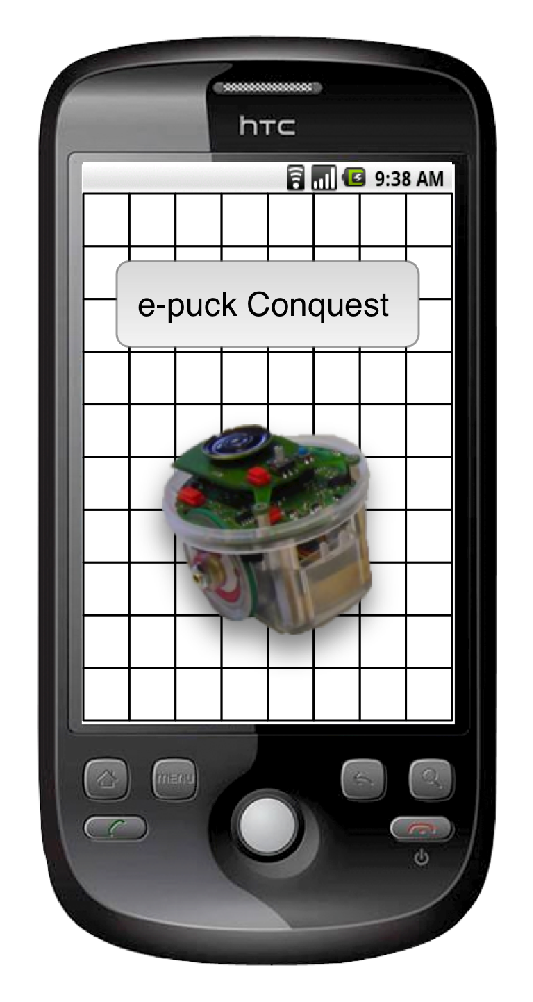
\includegraphics[height=10cm]{images/logo.eps} \\
	\vspace{1cm}
	Pflichtenheft
}
\author{SEP - ITS - Team \\ Max Binder, Florian Bürchner, Martin Freund, \\Florian Lorenz,
											Andreas Poxrucker, Andreas Wilhelm}
\begin{document}
	\date{22. Oktober 2010}
	\maketitle
	\newpage
	\tableofcontents	
	\newpage
	
	\section{Zielbestimmung}
		Das Ziel des Projekts ist die automatische Erkundung eines unbekannten, in Quadrate eingeteilten Spielfelds durch bis zu
		sechs e-puck Roboter. Die Erkundung soll durch Zusammenarbeit der Roboter möglichst effizient erfolgen.
		
		Das bereits erkundete Gebiet sowie die aktuellen Positionen der e-pucks werden mittels einer Anwendung auf einem Android
		Smartphone dargestellt.	
		
		Außerdem kann mit dem Smartphone einer der teilnehmenden e-puck Roboter ausgewählt und halbmanuell\footnote{Die
			möglichen Bewegungsrichtungen sind durch die Fahrbahnlinien eingeschränkt}  gesteuert werden.
		\subsection{Musskriterien}
			\begin{itemize}
				\item e-puck Roboter
				\begin{itemize}
					\item Variable Anzahl von Robotern
						\\ \textsl{Die Erkundung der Spielfläche kann durch bis zu sechs e-puck Roboter erfolgen.}
					\item Kommunikation über ein Bluetooth-Netzwerk
						\\ \textsl{Die Kommunikation der e-pucks untereinander erfolgt über ein Bluetooth-Netzwerk.
						   Dieses wird von den e-pucks selbstständig aufgebaut.}
					\item Erkundung einer unbekannten in Quadrate eingeteilten Fläche ausgehend von fest definierten Startpositionen
						\\ \textsl{Das Spielfeld besteht aus einer Menge von quadratischen \gls{Feld}ern. Diese sind rasterförmig
							und zusammenhängend angeordnet. Ein Feld ist mindestens 10cm x 10cm groß. Die Startpositionen der e-puck Roboter
						   sind fest vordefiniert.}
					\item Fortbewegung auf den Kanten der Quadrate
						\\ \textsl{Die Linien des Spielfeldes müssen schwarz mit ausreichendem Kontrastverhältnis
						    zum Untergrund sein. Zwingend erforderlich ist, dass die Breite der Linien innerhalb der Spezifikation der
							Bodensensoren liegt.}		
					\item Vermeidung von Kollisionen
						\\ \textsl{Während der Bewegung über das Spielfeld vermeiden die Roboter Kollisionen mit anderen Robotern.}	
					\item Gleichberechtigung der teilnehmenden Roboter
						\\ \textsl{Alle Roboter der Gruppe haben den selben Aufgabenbereich. Es gibt keine zentrale Einheit
							zur Koordination und Synchronisation.}	
					\item Einstellbare Geschwindigkeit
						\\ \textsl{Die Geschwindigkeit einzelner e-puck Roboter lässt sich vom Benutzer steuern. Insbesondere können Roboter
							zum Stillstand gebracht werden.}
					\item Dynamische Anpassung der Erkundung bei Deaktivierung / Ausfall einzelner Roboter
						\\ \textsl{Die erfolgreiche Erkundung des Spielfeldes ist gewährleistet, solange mindestens ein Roboter aktiv ist. Das 
							bedeutet, der e-puck wird nicht vom Benutzer angehalten oder manuell gesteuert. Außerdem müssen die
							unerkundeten Bereiche von ihm erreichbar sein.}
					\item Rückkehr zum Ausgangspunkt
						\\ \textsl{Nach Abschluss des Erkundungsvorgangs kehren alle Roboter zu ihren jeweiligen Startpositionen
							zurück.}	
				\end{itemize}
				\item Smartphone
				\begin{itemize}
					\item Kommunikation über Bluetooth
						\\ \textsl{Die Verbindung und Kommunikation mit den Robotern erfolgt über die Bluetooth-Schnittstelle des
							Smartphones.}
					\item Visualisierung
						\\ \textsl{Die bereits erkundeten Gebiete werden in einer benutzerfreundlichen Android-Anwendung übersichtlich
							dargestellt. Auf dieser Karte werden zusätzlich die aktuellen Positionen der e-pucks eingetragen.}
					\item Manuelle Steuerung eines Roboters
						\\ \textsl{Mit Hilfe der Anwendung kann einer der teilnehmenden e-pucks ausgewählt werden. Dieser lässt sich
							durch den Benutzer entlang der Linien in einstellbarer Geschwindigkeit steuern. Es kann jeweils nur ein Roboter
							zur selben Zeit ausgewählt und gesteuert werden.}		
					\item Zwei Steuerungsarten
						\\ \textsl{Die manuelle Steuerung der Roboter erfolgt wahlweise über einen On-Screen-Joystick oder über
							den im Handy integrierten Beschleunigungssensor.}											
				\end{itemize}
			\end{itemize}
		\subsection{Wunschkriterien}
			\begin{itemize}
				\item e-puck Roboter
				\begin{itemize}					
					\item Zustandsvisualisierung
						\\ \textsl{Die e-pucks stellen ihren aktuellen Zustand, zum Beispiel `Erkundung läuft' oder `Erkundung
							beendet', mit Hilfe der ihnen zur Verfügung stehenden Mittel dar.}										
					\item Beliebige Startpositionen
						\\ \textsl{Die Roboter können auf frei wählbaren Startpositionen innerhalb des Spielfeldes
							abgesetzt werden. Um dennoch Synchronisation zu erreichen ist ein erweiterter Lokalisierungsvorgang
							notwendig.}
					\item Einstellbarer Synchronisationsmodus
						\\ \textsl{Der Lokalisierungsmodus zwischen den e-puck Robotern lässt sich mit Hilfe des Programmselektors auswählen.}		
					\item Kritische Bereiche
						\\ \textsl{Auf dem Spielfeld gibt es Bereiche, in denen ein e-puck keine Nachrichten senden
							und empfangen darf. Diese Gebiete werden als `Kritische Bereiche' bezeichnet und müssen
							während des Erkundungsvorgangs besonders berücksichtigt werden.}									
				\end{itemize}
				\item Smartphone
				\begin{itemize}
					\item Anzeige von Statusinformationen
						\\ \textsl{Mit Hilfe des Smartphones ist es möglich, Informationen über den aktuellen Status der e-puck Roboter
							übersichtlich anzuzeigen.}		
					\item Pfadanzeige von Robotern
						\\ \textsl{Das Smartphone bietet die Möglichkeit den Pfad anzuzeigen, den jeder e-puck im Rahmen der
							Erkundung zurückgelegt hat.}							
					\item Exportfunktion für erkundete Karten
						\\ \textsl{Teilweise und vollständig erkundete Karten können in geeigneter Weise exportiert und auf dem
							Smartphone abgespeichert werden.}		
					\item Internationalisierung
						\\ \textsl{Die Anwendung ist in den Sprachen Deutsch und Englisch verfügbar.}									
				\end{itemize}
			\end{itemize}
		\subsection{Abgrenzungskriterien}
			\begin{itemize}
				\item Keine Unterstützung für abweichende Spielfelder
					\\ \textsl{Die Felder und zugehörigen Linien müssen den in den Musskriterien genannten Voraussetzungen
						genügen. Es sind zum Beispiel keine runden oder diagonalen Verbindungslinien erlaubt.}
				\item Keine Berücksichtigung von dynamischen Änderungen des Spielfeldes
					\\ \textsl{Nachdem der Erkundungsvorgang gestartet wurde, dürfen keine Modifikationen am
						Spielfeld getätigt werden, welche Einfluss auf den Erkundungsalgorithmus zur Folge hätten.
						Insbesondere werden keine nachträglichen Änderungen an bereits erkundeten Gebieten berücksichtigt.}			
				\item Unterstützung für maximal ein Smartphone
					\\ \textsl{Es kann lediglich ein Smartphone zur Auswahl, Steuerung und Visualisierung verwendet
						werden.}	
				\item Größe des Spielfeldes
					\\ \textsl{Der Arbeitsspeicher des e-puck Roboter stellt eine Obergrenze des speicherbaren Spielfeldes dar. }							
			\end{itemize}
	\section{Produkteinsatz}
		\subsection{Anwendungsbereiche}
			Das Projekt ist eine Forschungsarbeit in den Gebieten:
			\begin{itemize}
				\item Robotik
				\item Verteilte Systeme
				\item Künstliche Intelligenz
			\end{itemize}
		\subsection{Zielgruppen}
			Zielgruppen des Projektes sind insbesondere: 
			\begin{itemize}
				\item Studenten
				\item Forschungsgruppen in ähnlichen Bereichen
				\item e-puck Gemeinde
			\end{itemize}
		\subsection{Betriebsbedingungen}
			\begin{itemize}
				\item Ausreichende Stromversorgung
					\\ \textsl{Die Akkuleistung der einzelnen Roboter und des Smartphones muss für die gesamte
						Dauer der Lokalisierung, Erkundung und Rückkehr in die Startpositionen ausreichend sein.}
				\item Geeignete Bedingungen für Funknetzwerke
					\\ \textsl{Die Ausmaße des Spielfelds, die Abstände zwischen den e-pucks und zum Smartphone sowie
						Signale anderer Netze dürfen keine störenden Einflüsse auf die Bluetooth-Verbindungen haben.}
				\item Betriebsbedingungen der e-puck Roboter und des Smartphones
					\\ \textsl{Die weiteren Betriebsbedingungen können dem Benutzerhandbuch entnommen werden.}			
				\item Wartungsfrei
					\\ \textsl{Das System bedarf keiner regelmäßigen Wartung oder Aktualisierung.}	
				\item Namenskonventionen für das Bluetooth-Modul der e-puck-Roboter
					\\ \textsl{Die Kennung des Bluetooth-Modul der e-puck-Roboter muss zwingend folgender Namenskonventionen
						genügen: \textit{e-puck\_????} \footnote{ \ ? entspricht einer Ziffer}  }					
			\end{itemize}
	\section{Produktumgebung}
		\subsection{Software}
			\begin{itemize}
				\item Android Software ab Version 2.1
				\item CyanogenMod für Android Handys ab Version 6.0.1
			\end{itemize}
		\subsection{Hardware}
			\begin{itemize}
				\item e-puck Roboter (HW Rev. 2) mit Erweiterungsmodul für Bodensensoren
				\item Bluetooth fähiges Android Smartphone mit geeigneter Bildschirmauflösung, Touch-Display und optionalem
					Beschleunigungssensor zur Steuerung
			\end{itemize}		
		\subsection{Orgware}
			\begin{itemize}
				\item Tiny \gls{Bootloader} Version 1.97 zum Programmieren der e-puck Roboter
				\item Tiny Bootloader mit 16x \gls{PLL} für e-puck					
				\item PC ab MS Windows XP SP2 mit Bluetooth Modul
				\item APK-Installationsprogramm zur Übertragung der Anwendung auf das Smartphone per USB-Kabel \\
					(z.B. HTC Sync für HTC Geräte)
			\end{itemize}		
	\section{Produktfunktionen}
		\subsection{e-puck Roboter}
			\subsubsection{Netzwerkfunktionen}
				\begin{list}{\labelitemi}{\leftmargin=1cm}
					\item[\textbf{/F50/}] Suchfunktion
						\\ \textsl{Ein e-puck Roboter kann andere e-puck Roboter in Reichweite seines Bluetooth-Moduls entdecken.}
					\item[\textbf{/F60/}] Wahl der Kommunikationspartner
						\\ \textsl{Ein Roboter wählt beliebig einen anderen e-puck zum Aufbau einer Verbindung aus.}
					\item[\textbf{/F65/}] Verbindungsaufbau
						\\ \textsl{Die Verbindung wird zu dem ausgewählten Roboter (\textbf{/F60/}) aufgebaut und in die vorhandene
							Netzwerkstruktur integriert.}	
					\item[\textbf{/F70/}] Broadcast-Kommunikation
						\\ \textsl{Die e-puck Roboter können über bestehende Bluetooth-Verbindungen per Broadcast
						Nachrichten austauschen. Auch die Kommunikation mit dem Smartphone erfolgt via Broadcast.}
					\item[\textbf{/F75W/}] Kommunikationsunterdrückung
						\\ \textsl{Erreicht ein e-puck einen kritischen Bereich auf dem Spielfeld, kann er über bestehende
						Bluetooth-Verbindungen weder Nachrichten senden noch empfangen. Die Verbindungen an sich bleiben bestehen.}
				\end{list}
			\subsubsection{Bewegungsfunktionen}
				\begin{list}{\labelitemi}{\leftmargin=1cm}
					\item[\textbf{/F80/}] Grundbewegungen
						\\ \textsl{Der e-puck kann sich links und rechts um 90 oder 180 Grad drehen. Das Vorwärtsfahren erfolgt
							in Kamerarichtung des Roboters. Rückwärtsbewegungen entgegen der Kamerablickrichtung sind nicht möglich.}
					\item[\textbf{/F85/}] Einstellbare Fahrgeschwindigkeit
						\\ \textsl{Die Geschwindigkeit, mit welcher sich ein Roboter fortbewegt, kann stufenweise eingestellt werden. e-pucks
							können auch komplett angehalten werden. Eine Fortsetzung des Bewegungsvorgangs erfolgt durch erneute Erhöhung
							der Geschwindigkeit.}			
					\item[\textbf{/F90/}] Kollisionsvermeidung durch Austausch von Positionsinformationen
						\\ \textsl{Die Wegewahl eines e-puck Roboters wird durch Positionsangaben und Zielkoordinaten anderer Teilnehmer
							beeinflusst. Dadurch reduziert sich die Anzahl von möglichen Kollisionen.}		
					\item[\textbf{/F95/}] Kollisionsvermeidung durch Verwendung der Abstandssensoren
						\\ \textsl{Zusätzlich zu \textbf{/F90/} werden Informationen der integrierten Abstandssensoren verwendet, um
							bevorstehende Kollisionen zu vermeiden.}														
					\item[\textbf{/F100/}] Linienverfolgung
						\\ \textsl{Die e-pucks bewegen sich auf dem Spielfeld nur auf den vorhandenen Linien. Das gilt auch für e-pucks,
						die mit dem Smartphone halbmanuell gesteuert werden.}
					\item[\textbf{/F110/}] Knotenanalyse
						\\ \textsl{Ein e-puck erkennt beim Überfahren eines \gls{Knoten}s in welche Richtungen er weiterfahren kann.}
				\end{list}
			\subsubsection{Erkundungsfunktionen}
				\begin{list}{\labelitemi}{\leftmargin=1cm}
					\item[\textbf{/F120/}] Lokalisierung
						\\ \textsl{Vor Beginn des Erkundungsvorgangs einigen sich die e-pucks untereinander auf einen gemeinsamen Bezugspunkt
						und ermitteln relativ dazu ihre eigene Position. Die e-pucks starten in diesem Fall von fest definierten Startpositionen.}
					\item[\textbf{/F130/}] Auswahl des günstigsten zu erkundenden Knotens
						\\ \textsl{Jeder Roboter wählt selbständig den für ihn günstigsten noch nicht erkundeten Knoten.}
					\item[\textbf{/F135/}] Wegfindung und Fahrt zu bestimmten Knoten
						\\ \textsl{Die Roboter berechnen den Weg mit den geringsten Kosten zu einem bestimmten Knoten und bewegen sich
							anhand dieser Wegwahl dorthin.}
					\item[\textbf{/F140/}] Kartensynchronisation
						\\ \textsl{Während des Erkundungsvorgangs tauschen die e-pucks kontinuierlich Informationen über die von ihnen
						erkundeten Felder aus. Ist ein Smartphone mit dem Netzwerk verbunden, erhält auch dieses entsprechende Nachrichten.}
					\item[\textbf{/F150/}] Lokale Kartenkonstruktion	
						\\ \textsl{Jeder e-puck speichert lokal die bisher erkundete Karte. Diese wird mit Hilfe
						der Informationen aus den Nachrichten der anderen e-pucks sowie den eigenen Erkundungsergebnissen konstruiert.} 				
					\item[\textbf{/F155/}] Vollständigkeitserkennung 
						\\ \textsl{Die e-puck Roboter erkennen, dass das Spielfeld komplett erkundet wurde.} 	
					\item[\textbf{/F160/}] Rückkehrfunktion
						\\ \textsl{Nachdem das Gebiet vollständig erkundet worden ist, fahren die e-pucks wieder an ihre Startpositionen
						zurück.}
					\item[\textbf{/F170W/}] Globale Lokalisierung
						\\ \textsl{Starten die e-pucks nicht auf fest definierten Startpositionen, sondern auf beliebigen Feldern innerhalb
							des Spielfeldes, so können sich die Roboter durch vorher nicht festgelegte Treffpunkte untereinander lokalisieren.}
				\end{list}
		\subsubsection{Allgemeine Funktionen}
			\begin{list}{\labelitemi}{\leftmargin=1cm}
				\item[\textbf{/F180/}] Kalibrierung
					\\ \textsl{Die Linien- und Abstandssensoren lassen sich vom Benutzer manuell kalibrieren und dauerhaft abspeichern.}					
				\item[\textbf{/F190W/}] Zustandsvisualisierung		
					\\ \textsl{Der aktuelle Zustand (z.B. Kollisionen, manuelle Steuerung, synchronisiert) der einzelnen e-puck Roboter wird
						durch Verwendung verschiedener Aktoren und Außen-LEDs verdeutlicht.}		
			\end{list}
		\subsection{Smartphone}
			\subsubsection{Netzwerkfunktionen}
				\begin{list}{\labelitemi}{\leftmargin=1cm}
					\item[\textbf{/F200/}] Suchfunktion
						\\ \textsl{Das Smartphone entdeckt e-puck Roboter in Reichweite seines Bluetooth-Moduls.}
					\item[\textbf{/F205/}] Auswahl eines e-puck Roboters
						\\ \textsl{Der Benutzer kann am  Smartphone einen e-puck Roboter zum Aufbau einer Verbindung wählen.}						
					\item[\textbf{/F210/}] Verbindungsaufbau
						\\ \textsl{Das Smartphone kann sich via Bluetooth mit dem e-puck verbinden, der in \textbf{/F205/} ausgewählt
							wurde.}	
					\item[\textbf{/F220/}] Kommunikationsfunktion
						\\ \textsl{Das Smartphone kann über den verbundenen e-puck (\textbf{/F210/}) mit sämtlichen
							Netzwerkteilnehmern kommunizieren.}						
					\item[\textbf{/F225/}] Verbindungsabbau
						\\ \textsl{Die in \textbf{/F210/} aufgebaute Verbindung kann getrennt werden.}										
				\end{list}	
			\subsubsection{Erweiterte Funktionen}
				\begin{list}{\labelitemi}{\leftmargin=1cm}
					\item[\textbf{/F230/}] Statistikfunktion	
						\\ \textsl{Die eingehenden Daten der e-puck Roboter werden aufbereitet, sodass folgende Statistikinformationen für
							den Benutzer zur Verfügung stehen: 						
						\begin{itemize}
								\item Laufzeit der einzelnen e-puck Roboter
								\item Anzahl der erkundeten und befahrenen Knoten je e-puck
								\item Gesamtzahl der erkundeten und befahrenen Knoten	
								\item Gesamtverhältnis von erkundeten zu befahrenen Knoten
						\end{itemize}}				
					\item[\textbf{/F240W/}] Internationalisierung	
						\\ \textsl{Die Texte der Benutzeroberfläche werden abhängig von der gewählten Systemsprache des Smartphones
							angezeigt. Wird eine Sprache nicht unterstützt, so ist die Ausgabe standardmäßig englischsprachig.}
					\item[\textbf{/F250W/}] Kartenspeicherung	
						\\ \textsl{Die aktuell dargestellte Karte lässt sich auf dem Smartphone persistent abspeichern.}
					\item[\textbf{/F260W/}] Ladefunktion	
						\\ \textsl{Gespeicherte Kartendaten \textbf{/F250W/} können auf der Kartendarstellung des Smartphones geladen werden.}
				\end{list}						
			\subsubsection{Steuerungsfunktionen}		
				\begin{list}{\labelitemi}{\leftmargin=1cm}
					\item[\textbf{/F270/}] Steuerungsfunktion mit einem On-Screen-Joystick
						\\ \textsl{Der ausgewählte e-puck kann mit einem On-Screen-Joystick halbmanuell gesteuert werden. Die Bewegung
							erfolgt weiterhin auf den Linien des Spielfeldes. Die Geschwindigkeit kann stufenweise eingestellt werden. Die letzte
							Stufe stellt einen Stillstand des e-puck Roboter dar.}	
					\item[\textbf{/F280/}] Steuerungsfunktion mit dem eingebauten Beschleunigungssensor
						\\ \textsl{Alternativ kann der ausgewählte e-puck mit Hilfe des eingebauten Beschleunigungssensors halbmanuell
						gesteuert werden. Auch in diesem Fall bewegt sich der Roboter nur auf den Linien des Spielfeldes. Die Geschwindigkeit
						kann stufenweise eingestellt werden.}					
				\end{list}	
			\subsubsection{Funktionen der grafischen Benutzeroberfläche}
				\begin{list}{\labelitemi}{\leftmargin=1cm}
					\item[\textbf{/F290/}] Roboterauswahl durch Dropdown-Steuerelement
						\\ \textsl{Ein Roboter lässt sich durch die Auswahl eines Eintrages im Dropdown-Steuerlement auswählen.}					
					\item[\textbf{/F300/}] Roboterauswahl durch Kartenberührung
						\\ \textsl{Ein Roboter lässt sich alternativ über Berührung des entsprechenden e-pucks auf der Karte auswählen.}	
					\item[\textbf{/F310/}] Auswahl der Steuerungsart
						\\ \textsl{Der Benutzer hat die Möglichkeit über ein Dropdown-Steuerelement die Steuerungsart zu wählen. Zur Auswahl
							steht der On-Screen-Tasten-Joystick oder der  integrierte Bewegungssensor (gemäß \textbf{/F270/},
							\textbf{/F280/}).}
					\item[\textbf{/F320/}] Auswertung und Anzeige von Feldüberquerungen
						\\ \textsl{Es wird die Anzahl an Überquerungen je Feld gespeichert. Auf der Kartendarstellung erscheinen häufig befahrene
							Felder weniger transparent als selten befahrene.}	
					\item[\textbf{/F330/}] Autoskalierung der Karte
						\\ \textsl{Je nach Ausdehnung der Karte wird diese optimal auf dem Display dargestellt.}							
					\item[\textbf{/F340W/}] Zoomfunktion
						\\ \textsl{Der Benutzer kann mit Hilfe von Fingergesten in die Karte hinein bzw. heraus-zoomen. Der Kartenausschnitt
							kann hierbei verschoben werden.}										
				\end{list}		
	\section{Produktdaten}
		\begin{list}{\labelitemi}{\leftmargin=1cm}
			\item[\textbf{/D100/}] Kalibrierwerte
				\\ \textsl{Die Werte der Boden- und der Abstandssensoren werden nach dem Kalibrierungsvorgang dauerhaft abgespeichert.}
		\end{list}
		\begin{list}{\labelitemi}{\leftmargin=1cm}
			\item[\textbf{/D110W/}] Kartendaten
				\\ \textsl{Die aktuell dargestellte Karte kann zu jeder Zeit auf dem Android-Smartphone gespeichert werden.}
		\end{list}
		
	\section{Produktleistungen}
		\begin{list}{\labelitemi}{\leftmargin=1cm}
			\item[\textbf{/L50/}] Wiederaufbau der Bluetooth-Verbindung nach Verbindungsverlust
				\\ \textsl{Bei Verbindungsverlust eines Teilnehmers wird die Verbindung möglichst schnell wieder aufgebaut.}
			\item[\textbf{/L60/}] Robustheit des Systems bei Ausfall von e-puck Robotern
				\\ \textsl{Trotz des Ausfalls von einem oder mehreren Robotern kann der Betrieb fortgesetzt werden.}
			\item[\textbf{/L65/}] Gewährleistung der vollständigen Erkundung
				\\ \textsl{Solange sich mindestens ein e-puck Roboter im Erkundungsmodus befindet, nicht angehalten wird
					und der Zugang zu den unerkundeten Feldern zugänglich ist, wird die vollständige Erkundung gewährleistet.}		
			\item[\textbf{/L70/}] Möglichst effiziente Erkundung des Spielfelds
				\\ \textsl{Durch Zusammenarbeit mehrerer e-puck Roboter wird das Spielfeld möglichst effizient erkundet.}						
			\item[\textbf{/L80/}] Ungültige Richtungsanweisungen werden erkannt und nicht ausgeführt 
				\\ \textsl{Das System erkennt fehlerhafte Anweisungen des Benutzers und verweigert die Ausführung.}					
			\item[\textbf{/L90/}] Einarbeitungszeit 
				\\ \textsl{Die Benutzerschnittelle des Smartphones ist komfortabel und übersichtlich. Dadurch kann die Einarbeitungszeit
					auch für unerfahrene Benutzer kurz bleiben.}
			\item[\textbf{/L100/}] Unterstützte Spielfeldgröße 
				\\ \textsl{Die e-puck Roboter können ein Spielfeld mit bis zu 500 Knotenpunkten vollständig erkunden.}							
		\end{list}						
	\section{Benutzungsoberfläche}
	
			\subsection{Dialogstruktur}
			Im folgenden Schaubild wird die grundlegende Dialogstruktur der Android-Anwendung dargestellt.
			
			\begin{figure}[h]
				\centering
				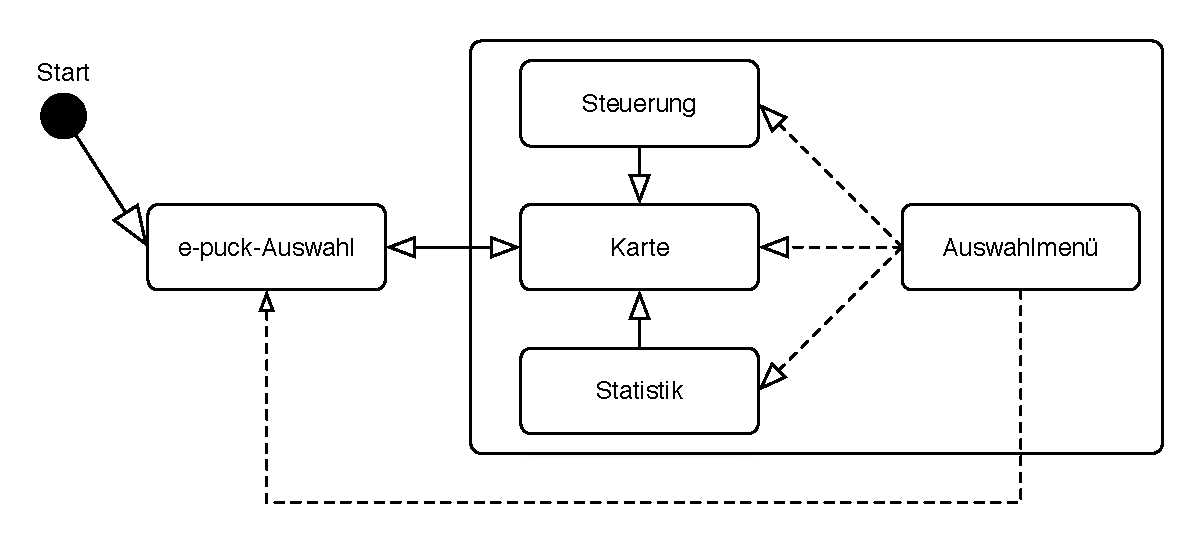
\includegraphics[width=10cm]{images/dialog.eps}
  				\caption{Dialogstruktur}
  			\end{figure}
  			
  			Nach Start der Anwendung kann der Benutzer wahlweise einen verbindungsbereiten e-puck Roboter auswählen oder eine
  			exportierte Karte laden. Daraufhin wird auf den Dialog 'Karte' gewechselt. \\
  			Über das Programm-Menü kann zwischen den Dialogen 'Steuerung', 'Karte' und 'Statistik' gewechselt werden. Befindet sich die
  			Anwendung auf dem Dialog 'Karte', so kann über die Zurück-Funktion die aktuelle Verbindung zu einem Roboter getrennt
  			und zur  e-puck-Auswahl gewechselt werden. Auf den Dialogen 'Steuerung' und 'Statistik' wird über die Zurück-Funktion
  			auf 'Karte' gewechselt.
  			
  			\subsection{Dialog 'e-puck-Auswahl'}
  			
			\begin{figure}[h]
				  \centering
				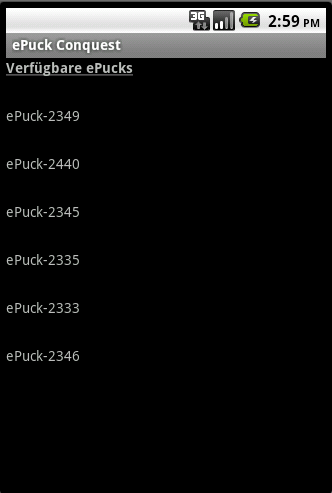
\includegraphics[width=3.5cm]{images/start.png}
				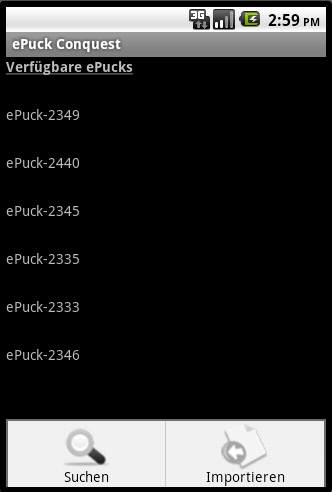
\includegraphics[width=3.5cm]{images/start_menu.png}
				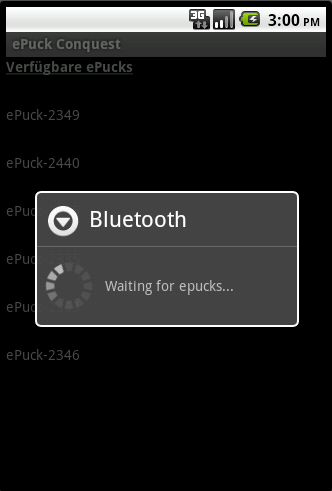
\includegraphics[width=3.5cm]{images/start_btsuche.png}
  				\caption{e-puck Auswahl}
  			\end{figure}	  				
  			
  				Beim Start der Anwendung wird dem Benutzer eine Auswahl der verbindungsbereiten e-puck Roboter angezeigt.  \\
  				Das Programm-Menü beinhaltet eine Funktion zum manuellen Start eines erneuten Suchlaufs, sowie eine Ladefunktion
  				für exportierte Kartendaten.
			
			\subsection{Dialog `Karte'}

			\begin{figure}[h]
				  \centering
				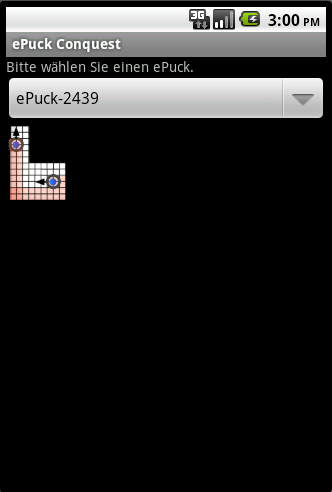
\includegraphics[width=3.5cm]{images/map.png}
				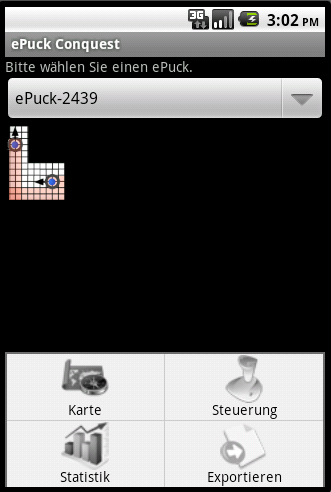
\includegraphics[width=3.5cm]{images/map_menu.png}
				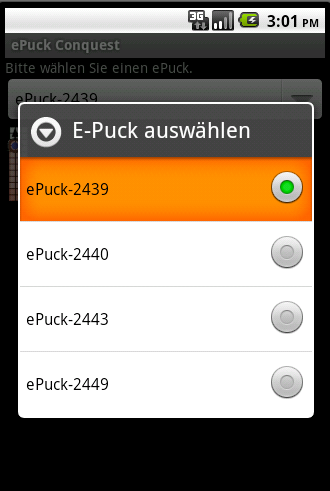
\includegraphics[width=3.5cm]{images/map_auswahl.png}
  				\caption{Kartendarstellung}
  			\end{figure}						
			
			Nachdem eine Kartensynchronisation (\textbf{/F140/}) stattgefunden hat bzw. wenn nur ein e-puck verfügbar ist, erfolgt die
			übersichtliche Darstellung des bereits erkundeten Gebiets auf einer Kartenansicht. Andernfalls wird keine Karte angezeigt.
			Je nach Ausdehnung der Karte wird diese optimal auf dem Display dargestellt. Außerdem werden die aktuellen Positonen der
			teilnehmenden e-pucks eingezeichnet. \\	
			Der Benutzer hat die Möglichkeit über Fingergesten in die Karte hinein- bzw. herauszuzoomen. Der Kartenausschnitt lässt sich
			hierbei beliebig verschieben. \\		
			Die Häufigkeit mit der ein Feld besucht wurde, wird durch die Transparenz des jeweiligen Feldes dargestellt. Häufig besuchte
			Felder sind hierbei weniger transparent als viel besuchte. \\
			Einer der e-pucks kann per Tippen auf die Kartendarstellung oder über das entsprechende Dropdown-Steuerlement ausgewählt
			werden. Dessen Position sowie die von ihm abgefahrenen Felder werden auf der Karte besonders hervorgehoben.\\
			Über das Programm-Menü kann der Benutzer auf die Dialoge 'Statistik' und 'Steuerung' wechseln.
			\subsection{Dialog `Steuerung'}
			
			\begin{figure}[h]
				  \centering
				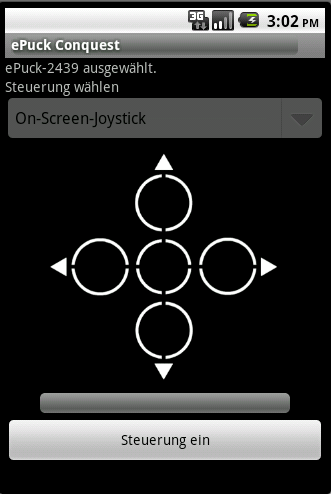
\includegraphics[width=3.5cm]{images/control.png}
				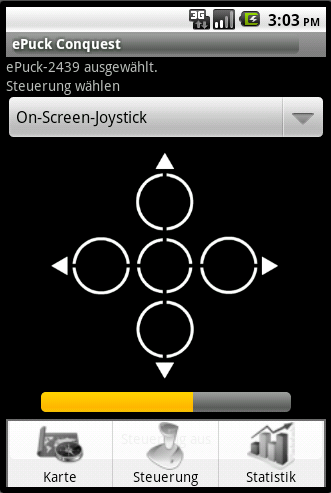
\includegraphics[width=3.5cm]{images/control_menu.png}
				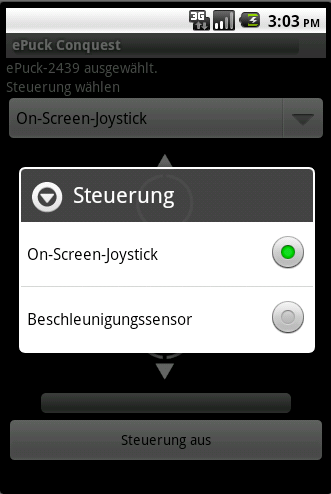
\includegraphics[width=3.5cm]{images/control_spinner.png}
				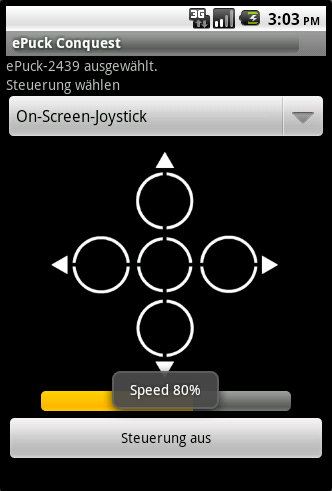
\includegraphics[width=3.5cm]{images/control_speed.png}				
  				\caption{Steuerungsarten}
  			\end{figure}	
			
			Die Ansicht `Steuerung' ermöglicht die halbmanuelle Steuerung eines e-puck. Die Auswahl erfolgt über das vorhandene
			Dropdown-Steuerelement. Dieses ist mit dem entsprechenden Steuerelement auf der Ansicht 'Karte' synchronisiert.	\\ 
			Der Benutzer kann die halbmanuelle Steuerung	aus- bzw. einschalten und zwischen den beiden beschriebenen
			Steuerungsarten über ein Dropdown-Steuerelement wählen. Es wird unabhängig von der gewählten Steuerungsmethode die selbe
			Oberfläche dargestellt. \\
			Über das Programm-Menü kann der Benutzer auf die Dialoge 'Karte' und 'Statistik wechseln.

			\subsection{Dialog `Statistik'}
				\begin{figure}[h]
					  \centering
					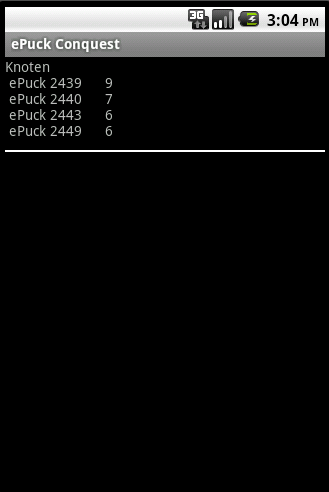
\includegraphics[width=3.5cm]{images/stats_bmp.png}
					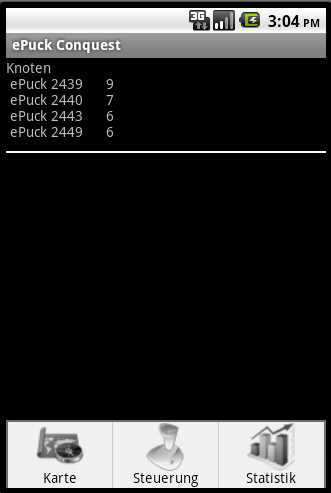
\includegraphics[width=3.5cm]{images/stats_menu.png}
  					\caption{Statistik}
  				\end{figure}		
  				
  			Die Ansicht `Statistik' zeigt Informationen gemäß \textbf{/F230/}. \\
  			
  			Über das Programm-Menü kann der Benutzer auf die Dialoge 'Karte' und 'Steuerung' wechseln.
			
	\section{Qualitätsbestimmungen}
		
		\subsection{e-puck Roboter}
			\begin{itemize}
				\item Effizienz
					\\ \textsl{Großer Wert wird auf eine hohe Performance des Systems gelegt. Dazu gehört insbesondere die effiziente Erkundung
						des Spielfelds. Die Nutzung des zur Verfügung stehenden Arbeitsspeichers erfolgt möglichst platzsparend.}
				\item Korrektheit
					\\ \textsl{Das unbekannte Spielfeld wird von den e-pucks vollständig und lückenlos erkundet.}
				\item Austausch- und Erweiterbarkeit
					\\ \textsl{Die Software-Architektur der e-pucks wird gezielt so entworfen, dass Komponenten der Logik einfach ausgetauscht
						und erweitert werden können.
						Dazu gehören neben der Fahr- und Steuerungslogik insbesondere die Mechanismen für Erkundung und Wegfindung.}	
				\item Robustheit 
					\\ \textsl{Das System wird so entworfen, dass die Erkundung des unbekannten Spielfeldes erfolgreich abgeschlossen
						wird, solange wenigstens ein e-puck nicht ausgefallen ist.
						Auch ein Ausfall des Smartphones führt nicht zum Abbruch des Erkundungsvorgangs.	}	
				\item Wartbarkeit
					\\ \textsl{Korrekturen im Softwaresystem können möglichst einfach durchgeführt werden.}				
			\end{itemize}		
		
		\subsection{Smartphone}
			\begin{itemize}
				\item Korrektheit
					\\ \textsl{Die Eingabedaten der e-puck Roboter werden vollständig und korrekt verarbeitet. Außerdem
						müssen die unterstützten Befehle in der Spezifikation entsprechenden Form versendet werden. Die grafische
						Benutzeroberfläche stellt die Daten korrekt dar.}
				\item Benutzerfreundlichkeit
					\\ \textsl{Die Anwendung ist einfach zu handhaben. Die Benutzeroberfläche ist übersichtlich und selbsterklärend. }
				\item Austausch- und Erweiterbarkeit
					\\ \textsl{Die Software-Architektur des Smartphones wird gezielt so entworfen, dass einzelne Komponenten, wie z.B. 
						Grafische Benutzeroberfläche oder Steuerungsfunktionalität, einfach ausgetauscht und erweitert werden können.}						
				\item Wartbarkeit
					\\ \textsl{Korrekturen im Softwaresystem können möglichst einfach durchgeführt werden.}			
			\end{itemize}
	
	\section{Globale Testszenarien und Testfälle}	
		Alle nachfolgenden Tests werden unter den genannten Betriebsbedingungen (Kapitel 2.3 Betriebsbedingungen)
		mit Hilfe einer Debug-Konsole durchgeführt.
			\begin{list}{\labelitemi}{\leftmargin=1cm}
				\item[\textbf{/T50/}] Kalibrierung
					\\ \textsl{Nach ordnungsgemäßer Kalibrierung beginnen die Außen-LEDs nacheinander zu leuchten (\textbf{/F180/}).}
				\item[\textbf{/T60/}] Linienerkennung
					\\ \textsl{Der e-puck wird im Betrieb entlang einer Linie aufgestellt und folgt dieser in Richtung der
						Liniensensoren (\textbf{/F100/}).}		
				\item[\textbf{/T70/}] Bluetooth-Scan
					\\ \textsl{Mehrere e-puck-Roboter werden auf dem Spielfeld platziert und eingeschaltet. Nach der Initialisierungsphase
						sollen sämtliche Teilnehmer auf dem Smartphone erkannt werden (\textbf{/F200/}).}		
				\item[\textbf{/T80/}] Broadcast-Test
					\\ \textsl{Gemäß \textbf{/T70/} werden alle verbindungsbereiten e-puck Roboter auf dem Suchdialog des Smartphone
						angezeigt. Es wird ein Roboter ausgewählt, alle im Netzwerk befindlichen Teilnehmer werden im Dropdown-Steuerelement
						aufgelistet  (\textbf{/F50/}, \textbf{/F60/}, \textbf{/F65/}, \textbf{/F70/}, \textbf{/F205/}, \textbf{/F210/}).}		
				\item[\textbf{/T90/}] Knotenanalyse und manuelle Steuerung per On-Screen-Joystick
					\\ \textsl{Der Roboter wird gemäß \textbf{/T60/} aufgestellt. Durch manuelle Steuerung per On-Screen-Joystick muss der
						Benutzer 	auf allen Knotentypen die möglichen Fahrtrichtungen testen. Nur gültige Richtungen
						dürfen vom Roboter befahren werden (\textbf{/F80/}, \textbf{/F110/}, \textbf{/F220/}, \textbf{/F270/}).}
				\item[\textbf{/T100/}] Steuerung der Fahrgeschwindigkeit
					\\ \textsl{Der Roboter wird gemäß \textbf{/T60/} aufgestellt. Bei der manuellen Steuerung per On-Screen-Joystick werden
						sämtliche Geschwindigkeitsstufen überprüft (\textbf{/F85/}).}					
				\item[\textbf{/T110/}] Steuerung per Beschleunigungssensor
					\\ \textsl{Der Test wird analog zu \textbf{/T80/} durchgeführt, wobei als Steuerungsmethode der Beschleunigungssensor
						verwendet wird (\textbf{/F280/}).}
				\item[\textbf{/T120/}] Erkundungstest
					\\ \textsl{Mehrere e-puck Roboter werden auf entsprechende Startpositionen innerhalb des Spielfelds gesetzt und
						eingeschaltet. Ziel des Testszenarios ist die vollständige Erkundung durch effiziente Zusammenarbeit der Teilnehmer.
						Falls die Roboter nach Abschluss auf die Startpositionen zurückkehren und die Karte auf dem Smartphone dargestellt
						wird, ist der Testfall erfolgreich (\textbf{/F90/}, \textbf{/F120/}, \textbf{/F130/}, \textbf{/F135/}, \textbf{/F140/},
						\textbf{/F150/}, \textbf{/F155/}, \textbf{/F160/}, \textbf{/F190W/}, \textbf{/F230/}, \textbf{/F320/}, \textbf{/F330/}).}
				\item[\textbf{/T130/}] Erweiterter Steuerungstest
					\\ \textsl{Der Benutzer wählt nach der Lokalisierung von mindestens zwei Roboter einen per Dropdown-Steuerelement aus.
						Anschließend wird die Steuerung über beide Steuerungsarten (\textbf{/F270/}, \textbf{/F280/}) durchgeführt. Im nächsten
						Schritt wird eine anderer Roboter gewählt und die Steuerung mit diesem geprüft (\textbf{/F290/}, \textbf{/F300/},
						\textbf{/F310/}).}
				\item[\textbf{/T140W/}] Speichern der Kartendaten
					\\ \textsl{Nachdem eine Kartenansicht auf dem Smartphone verfügbar ist, speichert der Benutzer die Kartendaten ab
						(\textbf{/F250W/}).}
				\item[\textbf{/T150W/}] Laden der Kartendaten
					\\ \textsl{Nachdem Kartendaten auf dem Smartphone gespeichert wurden (\textbf{/T120W/}), lädt der Benutzer diese.
						Daraufhin wird die entsprechende Karte angezeigt (\textbf{/F260W/}).}						
				\item[\textbf{/T160W/}] Test von globaler Lokalisierung
					\\ \textsl{Die e-puck Roboter werden im Gegensatz zu \textbf{/T110/} auf beliebigen Startpositionen gesetzt. Somit müssen
						sich die Teilnehmer zunächst finden und synchronisieren. Der erfolgreiche Abschluss kann durch die Anzeige aller e-pucks
						auf der Karte kontrolliert werden (\textbf{/F170W/}).}		
				\item[\textbf{/T170W/}] Test der Zoom-Funktionalität
					\\ \textsl{Nach dem Aufbau der Karte auf dem Smartphone werden Fingergesten zum Zoomen sowie Verschieben des
						Kartenausschnittes verwendet. (\textbf{/F340W/}).}																						
			\end{list} 
				
	%Glossar ausgeben
	\printglossary[style=altlist,title=Glossar]
						
\end{document}